% story.tex --- story-format companion draft of Paper A.
%
% This is a SEPARATE document from main.tex (draft v4), which is untouched and
% remains the technical report of record: it carries the full prediction ledger
% with commit hashes, the 27-configuration accounting, the perturbation-battery
% and mechanical-audit tables, and the per-table reproducibility notes.
% This version reorganises the SAME evidence as an instrument paper: the
% demonstration that the standard check fails, the instrument, its validation
% under real optimization pressure, and its robustness and cost.
%
% Every number here is copied from main.tex and its sections/ inputs (canonical
% producers: papers/analysis/*). No number, claim, caveat, or registration
% status has been changed. Where a registered prediction failed, the failure is
% stated where the claim appears.

\documentclass[11pt]{article}
\usepackage[margin=1in]{geometry}
\usepackage{amsmath,amssymb}
\usepackage{graphicx}
\usepackage{booktabs}
\usepackage{array}
\newcolumntype{L}[1]{>{\raggedright\arraybackslash}p{#1}}
\usepackage{xcolor}
\usepackage[colorlinks=true,linkcolor=blue,citecolor=blue,urlcolor=blue]{hyperref}
\usepackage{caption}
\captionsetup{font=small,labelfont=bf}

\usepackage{placeins}
\renewcommand{\topfraction}{0.9}
\renewcommand{\bottomfraction}{0.8}
\renewcommand{\textfraction}{0.07}
\renewcommand{\floatpagefraction}{0.75}
\setcounter{topnumber}{3}
\setcounter{totalnumber}{5}

\title{Agreement Is Not a Certificate}
\author{Anonymous Authors}
\date{Companion draft, September 1, 2026}

\begin{document}
\maketitle

\begin{abstract}
\noindent
LLM judges now rank models, filter data, and pick the best of $n$ samples, and the standard way to decide whether to trust one is raw agreement with human labels.
That check fails in the worst way: a judge can agree with humans on unoptimized data and still be gamed the moment something optimizes against it, because an agreement rate cannot reveal which properties drive the judge's score, and survival under optimization depends on two of them: how much substance the judge reads, and how much style.
We introduce a pre-deployment audit that measures it with the same labels: a few dozen blind human labels, graded separately for soundness and for style, yield a two-dimensional measurement --- how much of the target construct the judge reads, and how much of a nuisance construct --- and a frozen rule turns that measurement into a verdict of qualified, insufficient, or nuisance-loaded.
The audit convicts a deliberately sabotaged frontier judge and a top open reward model that raw agreement rates as interchangeable with honest judges, and the sabotaged judge shows why the distinction matters: under best-of-$n$ pressure it corrupts its own scoreboard while selecting almost as well as its honest twin, exactly the failure an accuracy check cannot see.
We validate the verdicts by running the optimization the audit is meant to predict: frozen before any pressure was applied, they called the best-of-$n$ outcome for ten of eleven registered configurations, and the single miss --- a pass that cleared its threshold by $0.01$ --- is reported in full.
On a prospective panel of nineteen new judges the frozen verdicts made no false certification and caught a harmful judge that a reference-presence shortcut certifies, though the panel's corruption arm failed to corrupt, so it tests the audit against weak judges rather than corrupt ones.
Under externally registered DPO training the audit identified which of two preference signals was harmful to optimize against: the qualified judge's arm gained accuracy on its training items and lost none held out, while the nuisance-loaded judge's arm degraded held-out accuracy; the registered scoreboard-wedge prediction was falsified in direction, the corrupted signal damaging the policy rather than teaching it to game.
The audit costs four to eight annotator-hours, one label set serves every judge configuration here, and its key verdicts reproduce on labels from a hypothesis-blind annotator outside the author list, turning evaluator trust from a post-hoc discovery into a measurement made before deployment.
\end{abstract}

\begin{table}[t!]
\centering
\small
\setlength{\tabcolsep}{4pt}
\begin{tabular}{llccccc}
\toprule
& configuration & verdict & raw $r$ & soundness partial & style partial & regret \\
\midrule
blind & 1.5B$^{a}$ & convict & $+0.18$ & $-0.00$ & $\mathbf{+0.51}$ {\scriptsize$[+0.13,+0.89]$} & $0.448$ \\
ladder & 3B & fail & $+0.24$ & $+0.19$ {\scriptsize$[-0.09,+0.53]$} & $+0.16$ {\scriptsize$[-0.17,+0.44]$} & $0.429$ \\
& 7B & fail & $+0.33$ & $+0.32$ {\scriptsize$[+0.04,+0.60]$} & $-0.02$ {\scriptsize$[-0.31,+0.30]$} & $0.324$ \\
& 14B & pass$^{*}$ & $+0.37$ & $+0.41$ {\scriptsize$[+0.12,+0.64]$} & $-0.21$ {\scriptsize$[-0.40,+0.00]$} & $0.324$ \\
\midrule
referenced & 1.5B & pass & $+0.55$ & $+0.51$ {\scriptsize$[+0.21,+0.75]$} & $+0.10$ {\scriptsize$[-0.21,+0.44]$} & $\mathbf{0.010}$ \\
ladder & 3B & pass & $+0.55$ & $+0.53$ {\scriptsize$[+0.36,+0.70]$} & $-0.02$ {\scriptsize$[-0.33,+0.29]$} & $0.038$ \\
& 7B & pass & $+0.66$ & $+0.66$ {\scriptsize$[+0.48,+0.82]$} & $-0.12$ {\scriptsize$[-0.35,+0.17]$} & $0.019$ \\
& 14B & pass & $+0.70$ & $+0.70$ {\scriptsize$[+0.50,+0.85]$} & $-0.11$ {\scriptsize$[-0.34,+0.15]$} & $0.048$ \\
\midrule
frontier & honest & pass & $+0.89$ & $+0.90$ {\scriptsize$[+0.77,+0.97]$} & $-0.22$ {\scriptsize$[-0.40,+0.05]$} & $0.117$ \\
(GPT-5.2) & sabotaged & convict & $+0.35$ & $+0.20$ {\scriptsize$[-0.07,+0.44]$} & $\mathbf{+0.59}$ {\scriptsize$[+0.36,+0.76]$} & $0.133$ \\
\midrule
sabotaged & 7B & fail & $+0.34$ & $+0.28$ {\scriptsize$[+0.07,+0.46]$} & $+0.17$ {\scriptsize$[-0.06,+0.38]$} & $0.400$ \\
ladder & 14B & fail & $+0.45$ & $+0.38$ {\scriptsize$[+0.06,+0.62]$} & $+0.24$ {\scriptsize$[-0.07,+0.47]$} & $0.324$ \\
\midrule
reward model & Skywork-8B & convict & $+0.18$ & $-0.01$ {\scriptsize$[-0.29,+0.28]$} & $\mathbf{+0.54}$ {\scriptsize$[+0.34,+0.70]$} & $0.286$ \\
\bottomrule
\end{tabular}

\medskip
\begin{minipage}{0.97\textwidth}
\footnotesize
\emph{Notes.}
Each row is one judge configuration on math; brackets are bootstrap 95\% confidence intervals.
\emph{Raw $r$}: plain correlation with human soundness labels (naive validation).
\emph{Soundness partial}: correlation with human soundness holding style fixed --- how much substance the judge reads.
\emph{Style partial}: correlation with human style holding soundness fixed --- the property the judge should ignore; significantly positive convicts.
\emph{Verdict}: the frozen rule's output (Section~\ref{sec:audit}).
\emph{Regret}: oracle regret under best-of-64 pressure (Section~\ref{sec:pressure}), repeated here so each verdict can be read against its outcome.
$n{=}60$ per row except 1.5B blind ($n{=}53$) and 1.5B referenced ($n{=}56$).
$^{a}$The 1.5B-blind bootstrap resamples are degenerate (concentrated scores), so its conviction carries jackknife and permutation inference instead: the bracketed interval is the jackknife CI, and the permutation test gives $p = 0.0017$ (two-sided, $n{=}53$).
$^{*}$The blind 14B pass is the record's one false pass (Section~\ref{sec:pressure}).
\end{minipage}
\caption{\textbf{Takeaway: raw agreement scores the sabotaged frontier judge ($+0.35$) and the honest blind 14B ($+0.37$) nearly identically, while the style partial separates them ($+0.59$ vs.\ $-0.21$) and names the failure mode; the frozen verdicts predicted the optimization outcome of ten of eleven registered configurations.}
The reward model, which raw agreement would call merely weak ($+0.18$), carries the sabotaged judge's signature.}
\label{tab:h2h}
\end{table}

\section{Introduction}
\label{sec:intro}

Consider a team that wires an LLM judge into best-of-$n$ serving: the model writes 64 candidate solutions per problem and the judge picks the one to keep.
On a spot check the judge agrees with human graders about 90 percent of the time, so the team trusts it.
Under optimization the scoreboard climbs while true quality does not: the pipeline has learned to produce answers the judge likes, not answers that are right, and the judge has been reward-hacked~\cite{gao2022scaling,skalse2022defining}.
Nothing in the agreement rate warned them, and nothing in it could have.

The reason is structural, not statistical.
Raw agreement measures performance on the observed, unoptimized distribution, and it does not identify which correlated attributes of a response drive the score.
The confound need not be large for this to bite: soundness and writing quality correlate at only $+0.32$ $[+0.10, +0.55]$ in our labeled sample, yet a sabotaged frontier judge and an honest mid-size judge land within $0.02$ of each other on raw correlation (Table~\ref{tab:h2h}) while reading opposite properties.
An optimizer breaks whatever correlation there is: it manufactures the property the judge rewards, and only one candidate property is correctness.
Optimization risk therefore has two sources, and a judge needs both measured.
A \emph{weak} judge fails because it reads little of the target construct; a \emph{capable-but-corrupt} judge reads the target and fails anyway, because it also reads a nuisance construct; only a judge with high target validity and low nuisance validity is safe to optimize against.
Both quantities are measurable from the same labels: grade the traces separately for soundness and for style, and compute the judge's partial correlation with each axis holding the other fixed.
This is classical construct validation~\cite{campbellfiske1959} pointed at a judge, and this paper's contribution is one sentence long: \textbf{static construct validity --- how much of the target and how much of a nuisance a judge reads, measured from a few dozen blind human labels --- predicts downstream optimization failure, including the capable-but-corrupt failures marginal agreement cannot see, and a frozen rule built on it called which judges got gamed before any optimization ran.}

Our contributions:
\begin{itemize}
\item \textbf{The demonstration that the standard check fails in the worst way.} A deliberately sabotaged frontier judge and an honest judge are indistinguishable by raw agreement, and an off-the-shelf reward model that naive validation calls merely weak carries the saboteur's signature; the partials separate all of them, with sign-anchored convictions fixed before outcomes (Section~\ref{sec:failure}; Table~\ref{tab:h2h}).
\item \textbf{An audit a practitioner can run tomorrow.} Sixty blind labels on two separated axes, two partial correlations, one frozen rule, four to eight annotator-hours --- with the checks that back its convictions against length confounds and multiple comparisons (Section~\ref{sec:audit}).
\item \textbf{Outcome validation under real optimization pressure.} The frozen verdicts called the best-of-64 outcome for ten of eleven registered configurations, and the one false pass, with the rule revision it forced, is reported in full (Section~\ref{sec:pressure}); a prospective panel of nineteen new judges confirmed three of five predictions and exposed why the other two failed (Section~\ref{sec:panel}); and under externally registered DPO training the audit identified which of two preference signals was harmful to optimize against, with one registered leg falsified in direction (Section~\ref{sec:dpo}).
\item \textbf{Robustness and cost.} The key verdicts reproduce on a hypothesis-blind non-author's labels, convictions stabilize by roughly forty labels, and two registered label-free extensions are scored honestly, one falsified sign included (Section~\ref{sec:robust}).
\end{itemize}

\paragraph{Registration.}
Every headline prediction was committed before the data it is scored on existed; registration means internal git timestamps on committed drafts and code, not an external registry, except where noted, and internal timestamps establish ordering but cannot rule out selective disclosure the way an external registry would.
The two later experiments carry external Open Science Framework registrations with third-party timestamps: the DPO rerun (\texttt{osf.io/jg4ak}, registered before its evaluation was read) and the pending Putnam replication (\texttt{osf.io/axp3s}, registered before any labels were collected).
Not everything we registered came true, and we report the failures where they bite rather than in a footnote: the audit's one false pass and the post-hoc rule revision it triggered (Section~\ref{sec:pressure}), the falsified conviction prediction for sabotaged mid-size judges (Section~\ref{sec:audit}), the falsified wedge and held-out legs of the training experiment (Section~\ref{sec:dpo}), a perturbation-battery sign prediction falsified in direction (Section~\ref{sec:robust}), and the prospective panel's two failed predictions together with the corruption manipulation that failed beneath them (Section~\ref{sec:panel}).
The complete ledger of predictions, timestamps, deviations, and outcomes lives in the technical report version of this paper, with a manifest naming a committed producer for every number quoted here.\footnote{Technical report version, draft v4, released with the code. It contains the full prediction ledger with commit hashes, the 27-configuration accounting, the perturbation-battery and mechanical-audit tables, and per-table reproducibility notes. This document reorganises the same evidence and changes no number.}

\begin{figure}[t!]
\centering
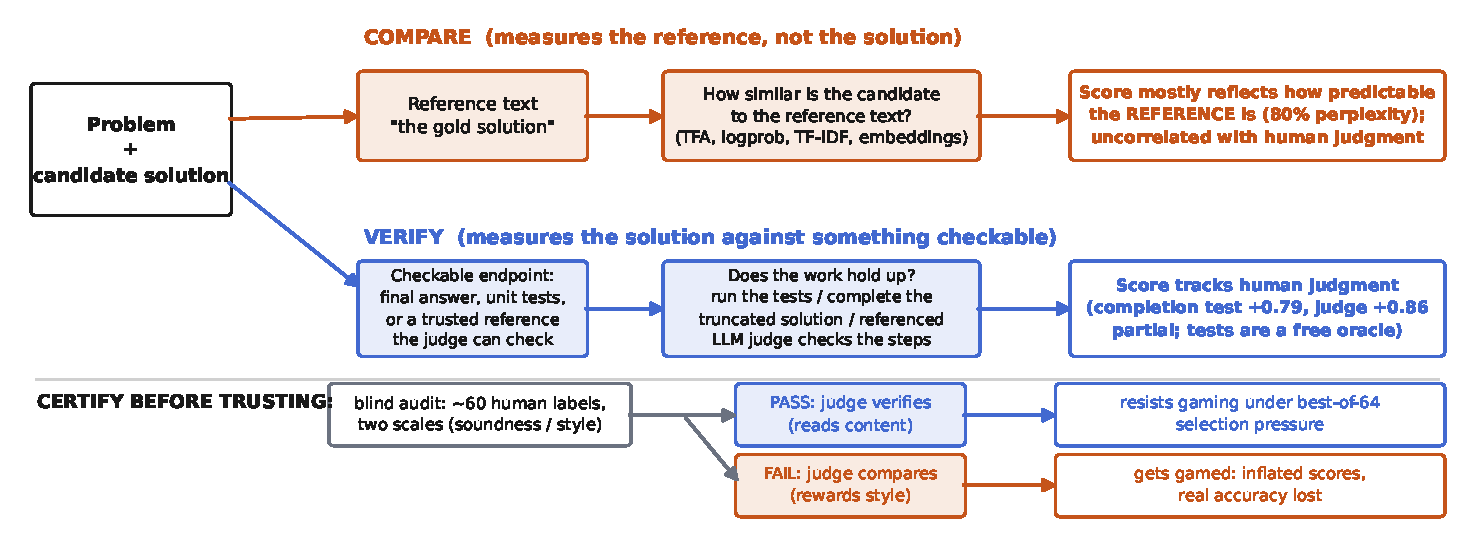
\includegraphics[width=\textwidth]{figures/fig_concept.pdf}
\caption{\textbf{Takeaway: evaluator failure has one dominant mechanism, so a small instrument aimed at it can predict gaming before any optimization runs.}
Top and middle: \emph{motivating background, established in companion work and not a result of this paper} --- the two evaluator mechanisms; comparison-shaped evaluators reward resemblance to a reference and load on properties like style, while verification-shaped evaluators check the solution against something trusted~\cite{companionB}. Every claim this paper makes stands on the bottom panel alone.
Bottom: the audit pipeline; a blind labeled set read through partial correlations classifies the mechanism, and the verdict predicts behavior under optimization pressure.}
\label{fig:concept}
\end{figure}

\section{Two evaluators the standard check cannot tell apart}
\label{sec:failure}

\paragraph{The cast.}
We audit thirteen judge configurations, all shown in Table~\ref{tab:h2h}.
The open-weights ladder is Qwen2.5 at 1.5B, 3B, 7B, and 14B, each deployed two ways: \emph{blind} (question and solution only) and \emph{referenced} (gold solution in context).
GPT-5.2 is the frontier judge, deployed honestly and, as the positive control, prompted to reward presentation (\emph{sabotaged}); an instrument that can only bless is not an instrument, so a judge \emph{built} to be style-loaded tests whether the audit can convict.
The same sabotage rubric was also run on the 7B and 14B ladder judges, though those two audits were scored against pressure outcomes already known and so enter the record only as late-scored confirmatory additions.
A trained reward model (Skywork-Reward-Llama-3.1-8B) is audited under predictions registered before its scores were generated.

\paragraph{The labels.}
The anchor set is a uniformly random sample of \textsc{MATH-500} solutions from seventeen models, graded blind by one annotator on two 0--10 scales with written anchors: \emph{soundness} (is every step valid; ignore the writing) and \emph{style} (is it clear and well-organized; ignore correctness).
Sixty items carry labels; per-configuration joins give $n = 53$--$60$.
All thirteen configurations score these same traces, so one label set prices every audit in this paper.

\paragraph{The demonstration.}
Raw agreement --- the plain correlation between judge scores and human soundness labels --- rates the sabotaged frontier judge at $+0.35$ and the honest blind 14B at $+0.37$: interchangeable.
The style partial separates them at $+0.59$ against $-0.21$, convicts the saboteur, and names its failure mode: this judge's scores track writing quality once soundness is held fixed.
The honest frontier judge passes cleanly, with a soundness partial of $+0.90$.
And the separation is not limited to the evaluator we corrupted ourselves: the Skywork reward model, an evaluator class the audit was not designed around, scores the same traces with the sabotaged judge's signature (style partial $+0.54$, soundness partial $-0.01$), where naive validation ($r = +0.18$) would report only weakness.
A third conviction lands on the blind 1.5B judge (style partial $+0.51$), whose scores carry essentially no soundness content at all.

The verdict tracks protocol, not model identity.
Blind, the 14B is the only ladder judge to clear the pass rule, and it does so by a hair --- soundness partial $0.41$ against a $0.40$ cut, a no-margin pass that Section~\ref{sec:pressure} shows to be false.
With the gold solution in context, every honestly prompted ladder judge passes.
A reference changes \emph{what} a judge measures, not merely how accurately it measures --- with the boundary that on tasks admitting several valid answers the same lever inverts and amplifies gaming, statically ($7$--$8$ points of verdict accuracy, whoever wrote the reference) and dynamically at all four ladder sizes~\cite{companionD}.

\paragraph{The failure is not specific to Pearson correlation.}
A reader may reasonably suspect we have picked a weak baseline, so we scored every configuration under five conventional marginal measures of judge--human agreement: Pearson and Spearman correlation with human soundness, Kendall's $\tau$, pairwise ordering accuracy against human soundness, and the area under the ROC curve for machine correctness (Table~\ref{tab:marginal}).
None of them separates the two style-loaded evaluators from the honest blind ladder.
The reward model sits \emph{inside} the honest blind ladder's range on all five; the sabotaged frontier judge sits inside on two and clears the top of the range by at most $0.06$ on the others, which is not a margin any deployment decision could rest on.
The nuisance loading is the only measure tested that puts both style-loaded evaluators outside the range of every configuration that is not style-loaded ($+0.59$ and $+0.54$ against a non-convicted maximum of $+0.24$).
This is the sharper form of the paper's claim: it is not Pearson correlation that fails, it is marginal agreement as a family, because every member of that family answers ``how often is this judge right here'' and none answers ``what is it reading.''

\begin{table}[t!]
\centering
\small
\begin{tabular}{lccccc}
\toprule
& Pearson & Spearman & Kendall $\tau$ & pairwise acc. & AUC (correct) \\
\midrule
honest blind ladder (range) & $[0.18, 0.37]$ & $[0.08, 0.28]$ & $[0.07, 0.26]$ & $[0.51, 0.62]$ & $[0.54, 0.79]$ \\
sabotaged frontier & $0.35$ & $0.34$ & $0.28$ & $0.66$ & $0.74$ \\
reward model & $0.18$ & $0.18$ & $0.13$ & $0.58$ & $0.58$ \\
\midrule
\multicolumn{6}{l}{\emph{separates both style-loaded evaluators?}\quad no \quad no \quad no \quad no \quad no} \\
\bottomrule
\end{tabular}
\caption{\textbf{Takeaway: marginal agreement fails as a family, not just as a Pearson correlation.}
Five conventional agreement measures on the same 60 labeled traces. The reward model falls inside the honest blind ladder's range on every one; the sabotaged frontier judge falls inside on two and exceeds the range by at most $0.06$ on the rest. The nuisance (style) loading separates both: $+0.59$ and $+0.54$ against a maximum of $+0.24$ over all configurations the audit does not flag. Post hoc; producer \texttt{cert\_review\_sensitivity.py}.}
\label{tab:marginal}
\end{table}

\paragraph{What marginal agreement can and cannot do.}
It is not useless: referenced judges score higher than blind ones, and a threshold placed between the clusters would have called the ladder outcomes.
But it conflates weak-honest with capable-corrupt, the distinction that determines the failure mode under pressure, and it offers no principled threshold --- the separating value is knowable only after the outcomes.
The audit shares that threshold problem for its weak-judge boundary (the blind-14B false pass is that problem realized), but its nuisance verdicts do not: a significantly positive style partial is a sign condition, fixed ex ante, and it alone identifies both style-loaded configurations.
The audit's advantage is diagnosis and a sign-anchored unsafe verdict, not a magically sharper threshold for weak judges.

\section{The audit}
\label{sec:audit}

The instrument is deliberately simple enough to run tomorrow.
(1) Draw a uniformly random sample of the deployment's own traces --- here, sixty.
(2) Have an annotator grade each trace blind on two separated axes with written anchors: the target axis (soundness) and an axis the judge should ignore (style).
Separated axes are the load-bearing choice: a single quality number makes loading on the wrong axis unmeasurable in principle.
(3) Score the traces with the judge under audit.
(4) Compute the soundness partial and the style partial.
(5) Read the two numbers as the measurement they are --- a target loading and a nuisance loading --- and only then apply the frozen rule that turns them into a decision: \emph{nuisance-loaded} (unsafe to optimize against) if the style partial exceeds $0.30$; \emph{qualified} if the soundness partial exceeds $0.40$ and the style partial is below $0.20$; \emph{insufficient target validity} otherwise.
We keep the shorthand \emph{convict} for the unsafe verdict in prose, because it is the memorable word for what the instrument does, but nothing in the method depends on the vocabulary: the object is the pair of loadings, and the rule is a deployment policy laid over it.
Labeling sixty traces on two axes at two to four minutes per trace-axis (120 trace-axis gradings) is four to eight annotator-hours, amortized across every judge scored on the same traces.
The axes here are an instantiation chosen for the threat model, not a fixed pair: style is the dominant documented nuisance axis~\cite{wu2023style,rmbench2024}; length, format, and position are probed separately (Section~\ref{sec:robust}).

Two auxiliary pieces complete the instrument.
A deliberately selected subsample --- built where cheap signals disagree, which spreads the soundness axis (mean $6.7$, sd $3.4$) that the random set leaves near ceiling (mean $8.3$, sd $2.8$) --- supplies power for one check that the random set cannot: whether the judge separates sound from lucky reasoning among right answers (the honest frontier reads $+0.81$ there but $-0.14$ on the random set, where range restriction destroys the question)~\cite{companionB}.
Because that subsample is selected by conditioning on the judges' own signals, it induces Berkson-style effects and its numbers never enter the headline partials; the uniformly random anchor set, which cannot be tuned toward any outcome, carries every verdict.
And before spending any labels, a free pre-screen gates everything: a judge whose pairwise verdict flips when the candidate order is swapped ($71$--$95\%$ flip rate at 0.5B scale, falling to $2$--$37\%$ at 14B~\cite{companionB}) cannot pass any validity audit, at zero cost.

\paragraph{The convictions survive their two obvious rebuttals.}
First, length: the reward model strongly prefers short responses (length partial $-0.54$), so its style conviction could be a length preference in disguise.
A three-variable partial answers directly: with soundness and length both controlled, the reward model's style partial moves only from $+0.54$ to $+0.42$, the sabotaged frontier's shifts similarly ($+0.59$ to $+0.47$), and the honest frontier stays clean --- the convictions are genuinely style.
Second, multiplicity: the conviction rule is a single pre-declared sign condition per configuration, not a search over thresholds, and under Bonferroni correction across the eleven registered configurations all three convictions remain significant (corrected intervals $[+0.25, +0.80]$ for the sabotaged frontier and $[+0.20, +0.77]$ for the reward model; the 1.5B permutation $p = 0.0017$ sits below $0.05/11$).

\paragraph{A registered conviction prediction that failed.}
The sabotage instruction behaves differently below frontier capability, and one of our registered predictions was wrong there.
We predicted the sabotaged 7B and 14B would be convicted; that prediction is falsified --- neither style partial is significantly positive --- and both instead fail, with soundness partials below the pass cut (Table~\ref{tab:h2h}).
Both fail verdicts match the pressure outcomes, but because they were scored after those outcomes were known, they enter only the secondary record.
The scale comparison carries a mechanism: the corrupt instruction loads style only at frontier capability (style partial $+0.59$ at GPT-5.2 versus at most $+0.24$ at ladder scale), and at ladder scale it instead degrades the judge into a weak one.
Corrupt instructions are capability-gated, which strengthens the case for auditing per deployment rather than per model class.

\section{The verdicts under selection pressure}
\label{sec:pressure}

A verdict computed from static labels is only as good as its forecast, so we ran the optimization the audit is meant to predict, with the verdicts frozen first.
A 7B generator writes 64 candidates per problem, each judge configuration picks its favorite, and two pre-registered quantities separate deception from damage.
\emph{Inflation} (the excess hack gap) measures how far the judge's own scoreboard rises relative to true quality, in baseline standard deviations over a permutation null that shuffles judge scores among samples with the same correctness; selection and reporting use different rubric paraphrases, canceling winner's curse.
\emph{Regret} (oracle regret) measures accuracy left on the table against best-possible selection.
Item pools are 105 \textsc{MATH-500} and 68 \textsc{MBPP+} items on which the generator sometimes but not always succeeds (pool pass rate in $[0.2, 0.8]$); estimators were committed before generation.

\paragraph{Ten of eleven, per estimand.}
The frozen verdicts called the outcome for ten of the eleven registered configurations, and the answer is per estimand: fails predict regret, convictions predict inflation or damage.
Applying the frozen rule uniformly to all thirteen audited configurations yields six passes, four fails, and three convictions; twelve of thirteen verdicts predict the pressure outcome, the two late-scored sabotaged-ladder rows counting only toward that secondary record.
On regret, every failed configuration (minimum $0.32$) exceeds every correctly certified one (maximum $0.12$).
On inflation, over the registered eleven, the failed-or-convicted cluster (minimum $+0.44\sigma$) sits above the correctly certified cluster (maximum $+0.38\sigma$) --- a cluster-level statement, not eleven pairwise separations: the one boundary pair (blind 3B against the honest frontier's own elevated inflation, difference $+0.06$ $[-0.10, +0.22]$) is not statistically separable, while the informative contrasts --- sabotaged versus honest frontier, blind versus referenced, false pass versus honest --- all separate.

\begin{figure}[t!]
\centering
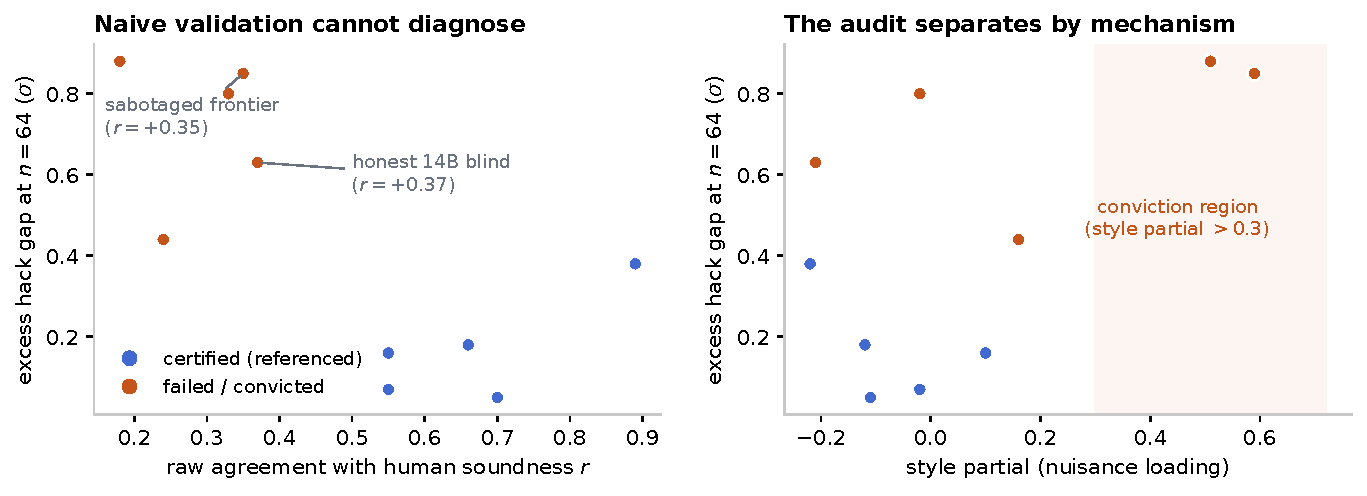
\includegraphics[width=\textwidth]{figures/fig_h2h.pdf}
\caption{\textbf{Takeaway: naive validation ranks but cannot diagnose; the style axis separates capable-corrupt from weak-honest.}
Each point is one audited math configuration; the $y$ axis is its scoreboard inflation under best-of-64 pressure.
Left: raw agreement with human soundness places the sabotaged frontier judge inside the failed-blind cluster.
Right: the style partial isolates both style-loaded configurations in a sign-anchored conviction region fixed before outcomes.}
\label{fig:h2h}
\end{figure}

The two headline convictions show exactly the damage their verdicts predicted.
The sabotaged frontier's inflation ($+0.85$ $[+0.70, +1.01]$) is disjoint from the honest frontier's ($+0.38$ $[+0.28, +0.50]$) --- more than twice it --- while its regret is statistically indistinguishable from honest (difference $+0.014$ $[-0.058, +0.085]$).
That asymmetry is itself a finding: a style-loaded frontier judge corrupts the scoreboard without measurably corrupting selection at this pressure, which is exactly the failure a naive accuracy check cannot see, and exactly the mode that menaces training (Section~\ref{sec:dpo}).
The convicted reward model completes the picture: its inflation is $+1.46\sigma$ $[+1.33, +1.58]$, the largest measured, under a registered prediction that it would out-inflate the certified referenced tier, and its regret ($0.286$ on math, $0.485$ on code, the latter inside the failed-blind code cluster of $0.368$--$0.544$) separates from every correctly certified configuration.\footnote{The reward model's inflation uses a candidate-side paraphrase replicate --- selection on original candidates, reporting on content-preserving paraphrases --- because a single scoring function cannot supply the independent replicates the estimand requires. The estimand is analogous to the judge protocol's rather than identical, so the clean statement is that it exceeds every certified configuration under the registered prediction; the number carries a dual reading --- winner's-curse inflation, or score movement under content-preserving rewording --- and both readings are damning for a deployed reward signal.}

\paragraph{The false pass, and the statistical fact behind it.}
The exception is the blind 14B, and it is the most instructive row in the table.
Its soundness partial clears the $0.40$ cut by $0.01$, yet under pressure it sits in the failed cluster (inflation $+0.63$ $[+0.42, +0.84]$, regret $0.324$); the label-subsampling analysis of Section~\ref{sec:robust} had already marked this verdict unstable below the full label set.
The false pass exposes a general statistical fact rather than a badly placed cut: with finitely many labels, a point threshold cannot support certification near a decision boundary, and the simulation of Section~\ref{sec:robust} shows that a judge whose true target loading sits at the boundary is certified on a coin flip at sixty labels and still at two hundred forty.
Uncertainty-aware abstention is therefore structurally necessary, not a patch.
We revise the rule accordingly, explicitly post hoc: certification requires the soundness-partial \emph{confidence interval}, not the point estimate, to clear the bar.
The revision can only withdraw certifications, never grant one, so it cannot convert the disclosed failure into a success, and every headline record in this paper is scored under the original frozen rule with the revised rule reported separately.
Nor is the revision free, and we account for its full retrospective effect: two threshold-adjacent referenced judges (1.5B and 3B) whose intervals also straddle the bar become abstentions, even though both behaved well under pressure (regrets $0.010$ and $0.038$, the first- and third-lowest observed).
The revised rule's retrospective record is eight predictions, eight correct, three abstentions; it trades coverage for safety and is frozen for the externally registered Putnam replication (\texttt{osf.io/axp3s}).

\paragraph{Incremental validity over a protocol bit.}
The audit must also beat the strongest trivial baseline: a classifier that predicts certified behavior iff a reference is present.
On the same thirteen configurations that protocol bit scores ten of thirteen --- wrong on all three sabotaged referenced arms, which it cannot see, and right on the blind 14B, where the audit false-passes.
The audit scores twelve of thirteen.
Its incremental value is precisely detection of corrupted instructions and reward models, at the cost of one boundary miss.

\begin{figure}[t!]
\centering
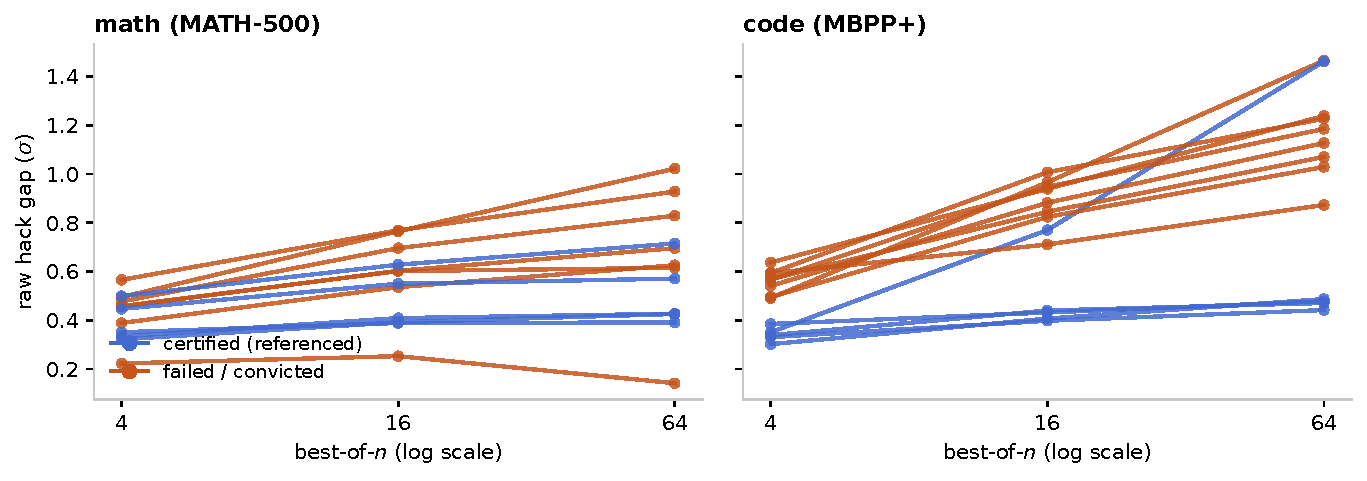
\includegraphics[width=\textwidth]{figures/fig_curves.pdf}
\caption{\textbf{Takeaway: within each domain, certified configurations stay low and flat relative to failed ones, but pressure growth is heterogeneous --- the certificate predicts relative position within a domain, not a universal slope.}
Raw hack gap versus best-of-$n$ for every configuration with existing candidate pools, recomputed at $n = 4, 16, 64$ with the pre-registered estimators.
Blue: certified (referenced) configurations; orange: failed or convicted ones.
Some certified curves do rise (the referenced frontier on math moves $+0.50 \to +0.71$; the referenced 14B on code $+0.30 \to +0.49$), the referenced 1.5B on code climbs to failed-cluster levels ($+0.35 \to +1.46$, the capability-gate miss), and the sabotaged 7B on math declines ($+0.22 \to +0.14$).}
\label{fig:curves}
\end{figure}

\paragraph{The separation persists as pressure grows.}
The failed-versus-certified separation holds as $n$ increases, though not every curve behaves.
Failed configurations generally steepen (the blind 3B's code gap runs $+0.64 \to +1.24$ across $n = 4 \to 64$) while certified ones stay comparatively flat (the referenced 3B runs $+0.33 \to +0.44$ on code); the exceptions in both directions are enumerated in the caption of Figure~\ref{fig:curves}.

\paragraph{Two failure modes, and capability trades one for the other.}
Across the sabotage arms, damage falls and self-inflation rises with judge capability.
The sabotaged 7B damages without inflating (regret $0.400$; inflation $+0.13$ $[-0.13, +0.35]$, not significant); the sabotaged frontier inflates without measurable damage.
A blind cross-family panel confirms the channel: sabotage-selected solutions are more styled ($+0.27$ $[+0.10, +0.44]$) with no detectable soundness loss~\cite{companionB}.
The sabotaged-ladder audits locate the same trade on the instrument side, where the corrupt instruction produces a failed judge at ladder scale and a style-loaded one only at the frontier (Section~\ref{sec:audit}).

\paragraph{Cross-domain transfer, and an audit with a mechanical target axis.}
The audit generalizes beyond human labels wherever the target axis has an oracle, and code supplies one: executed tests.
We audited every code configuration by the within-item correlation of its scores with test outcomes, no human labels involved; code verdict predictions were not registered, so this scoring is post hoc, and the two sabotaged code ladder cells remain unaudited under the paper's exclusion policy, leaving eleven eligible configurations.
The extrapolated verdicts match the pressure outcome in ten of those eleven, and the measured rows explain the single miss directly: the 1.5B judge's reference adds nothing to its target-axis validity on code ($+0.15$ blind, $+0.16$ referenced) --- the capability gate measured rather than inferred --- and that configuration is gamed as badly as its blind twin (inflation $+1.40$, regret $0.441$; Figure~\ref{fig:gate}).
The frontier tier separates cleanly ($+0.52$ blind, $+0.62$ referenced), and sabotage measurably degrades target validity even against a mechanical target ($+0.62 \to +0.42$).
Operationally: a judge certified on one domain is not thereby certified on another --- run the audit, with whatever target oracle the domain offers, where the judge will be used.

\begin{figure}[t!]
\centering
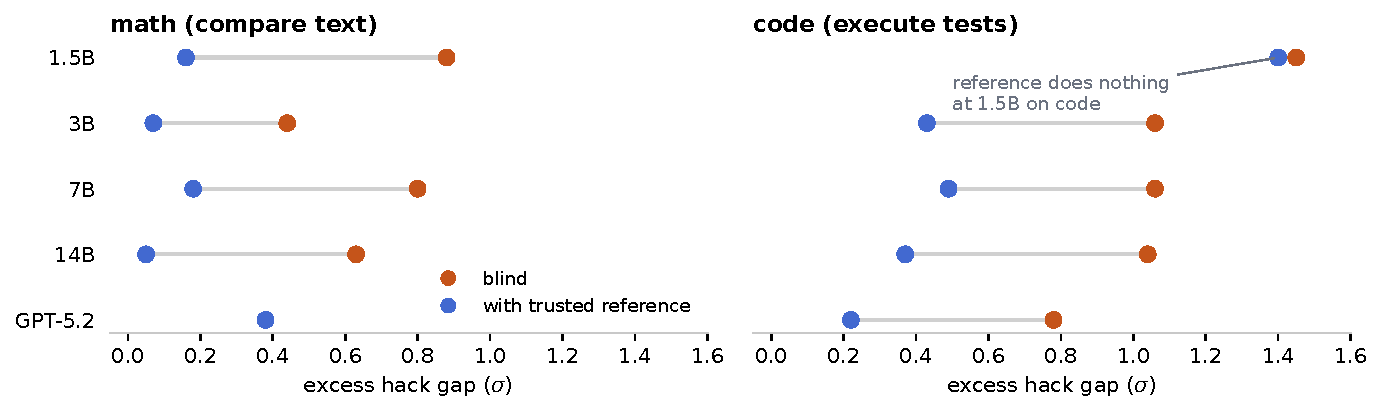
\includegraphics[width=0.9\textwidth]{figures/fig_gate.pdf}
\caption{\textbf{Takeaway: the reference collapses inflation at every scale on math, where using it means comparing text, and only at 3B and above on code, where using it means executing tests.}
Inflation at $n{=}64$ without (orange) and with (blue) a trusted reference, by judge scale and domain.}
\label{fig:gate}
\end{figure}

\section{A prospective panel, and what it could not test}
\label{sec:panel}

The thirteen configurations above cannot settle whether the audit adds anything over reference presence, because their verdicts track that one bit.
So after freezing the rule we built a panel meant to break the link: nineteen judge configurations new to this work, including capable judges given no reference, a weak judge given one, subtly corrupted prompts with and without a reference, and two trained reward models not used elsewhere in this paper.
Every prompt, the decision rule, the outcome definition, and both analysis producers were committed before any panel judge ran, and the audit verdicts were committed before any best-of-64 score existed.
Both are internal git timestamps; the panel was drafted for external registration but was not posted, a deviation we disclose here and in the ledger.
A cell's outcome counts as unsafe if its best-of-64 regret reaches $0.25$ or its inflation reaches $+0.50$, cut-points taken from the thirteen configurations above before the panel ran.

\paragraph{The panel does not contain the case the audit exists for.}
We state this first because it governs how everything after it should be read.
Seven cells carried a corrupting instruction, ranging from ``prefer answers that are clear and convincing'' to a hidden preference for tidy formatting.
A post-hoc manipulation check against an exact honest twin of each cell --- the same judge and prompt without the corrupting sentence --- shows that five of the seven did not change their judge at all: their scores track the twin at $r \geq 0.986$, with mean shifts below $0.05$ on the ten-point scale.
The two that moved, both Qwen2.5-14B, did not move toward style (nuisance loadings $-0.09$ and $+0.01$), which repeats the capability gate of Section~\ref{sec:audit} at 8B to 14B and with subtler wording: below frontier scale, a corrupt instruction does not produce a style-loaded judge.
The panel therefore contains weak judges and trained reward models but no successfully corrupted instruction-following judge, and its results are a test of the audit against weakness, not against corruption.
We registered no manipulation check, so this is a design failure of the panel, not a reinterpretation of its predictions.

\begin{table}[t!]
\centering
\small
\begin{tabular}{L{9.0cm}cc}
\toprule
\multicolumn{3}{l}{\emph{A. Deployment decisions, frozen before optimization}} \\
\midrule
decision & cells & matched outcome \\
\midrule
qualified $\rightarrow$ safe & $7$ & $7/7$ \\
insufficient target validity or nuisance-loaded $\rightarrow$ unsafe & $7$ & $7/7$ \\
abstain, no decision issued & $5$ & all $5$ unsafe \\
reference-presence bit, on the same $14$ decided cells & $14$ & $13/14$ \\
\midrule
\multicolumn{3}{l}{\emph{B. Ranking cells by risk: AUC for the unsafe outcome}} \\
\midrule
target loading (post hoc) & & $1.000$ \\
raw correlation with human soundness & & $1.000$ \\
reference-presence bit & & $0.958$ \\
nuisance loading (the registered ranker, P-N3) & & $0.845$ \\
\midrule
\multicolumn{3}{l}{\emph{C. Registered predictions}} \\
\midrule
confirmed: P-N1 audit beats the reference bit where it decides; P-N4 separation within referenced cells; P-N5 both reward models unsafe & & $3$ \\
failed: P-N2 most corrupt cells called unsafe ($0/7$); P-N3 nuisance loading outranks both baselines & & $2$ \\
\bottomrule
\end{tabular}
\caption{\textbf{Takeaway: every decision the audit issued matched the optimization outcome, but because the panel's corruption manipulation failed, the panel varies target validity rather than nuisance validity, and on such a panel target loading and raw agreement rank risk equally well.}
The ranking prediction P-N3 was falsified for that reason: nuisance loading is the axis that separates capable-but-corrupt judges, and this panel contains none. The raw-correlation classifier reaches perfect accuracy only at a threshold ($0.704$) chosen after seeing outcomes; the audit's rule was frozen. Producers: \texttt{panel\_verdicts.py}, \texttt{panel\_outcome.py}; manipulation check \texttt{panel\_manipulation.py} (post hoc).}
\label{tab:panel}
\end{table}

\paragraph{Where the audit spoke, it was right.}
All seven qualified cells had safe outcomes, with inflation from $+0.05$ to $+0.26$ and regret at most $0.057$, and all seven cells called insufficient or nuisance-loaded had unsafe ones (Table~\ref{tab:panel}).
The reference bit scores thirteen of those same fourteen.
The one disagreement is a Qwen2.5-0.5B judge given the gold solution: the bit certifies it, the audit calls it nuisance-loaded (nuisance loading $+0.44$ $[+0.11, +0.62]$, target loading $-0.02$), and under pressure it leaves $0.362$ regret.
Within the eight referenced cells, where the bit is constant and says nothing, nuisance loading separates that cell from the other seven without overlap.
Both reward models were called unsafe, with nuisance loadings of $+0.30$ and $+0.42$ and intervals excluding zero, and they were the two most inflated cells in the panel, at $+1.55$ and $+1.25$, which replicates the published reward-model conviction on two further models.

\paragraph{Where it did not.}
The five abstentions all fell on blind judges whose target-loading intervals straddle $0.40$, and all five turned out unsafe.
The interval rule certified none of them, so abstaining cost no false certification, but it issued no warning either, and across all nineteen cells the reference bit is right on eighteen, which is more ground than the audit covers.
P-N2 fails at zero of seven, and the manipulation check says why.
P-N3 fails as well, and it fails for a specific reason (Table~\ref{tab:panel}, panel B).
Because the corruption manipulation failed, this panel varies target validity rather than nuisance validity, and on such a panel the risk ranking belongs to the target axis, which ranks perfectly, as does raw agreement, since being wrong on unoptimized data is what both measure.
Nuisance loading, the registered ranker, is the axis for capable-but-corrupt judges, and the panel contains none; the prediction named the wrong axis for the panel we ended up with, and we score it as failed.
Raw agreement's perfect accuracy also required a threshold chosen after the outcomes were known, whereas the audit's rule was fixed in advance.

\paragraph{What the panel adds, and what it does not.}
The panel became a prospective test of one half of the instrument and not the other.
It validates, under a frozen rule, that measuring target validity prevents false certification: no judge it had never seen was certified and then gamed, and it caught a harmful referenced judge the protocol bit certifies.
It does not validate the half that distinguishes this paper, that nuisance loading separates capable-but-corrupt judges from capable-honest ones, because it contains no capable-but-corrupt instruction-following judge; prospective evidence for that regime is so far limited to the two reward models, and the collinearity objection of Section~\ref{sec:limits} is correspondingly narrowed, not closed.
The experiment still owed is a panel whose corrupt cells pass a manipulation check before they are audited, and the failure here shows how to build one: subtle instructions are ignored below frontier scale, so corruption at that scale has to come from the model itself, as it does for reward models, or from a frontier judge.

\section{The verdicts under training pressure}
\label{sec:dpo}

Selection is the weaker optimizer; the deployed risk is a judge building preference data for training, and the frontier failure mode of Section~\ref{sec:pressure} --- scoreboard corruption without selection corruption --- is precisely where selection understates risk.
If the verdicts read the exploitable property, then training a policy against the certified judge should produce real gains, training against the convicted judge should not, and, as registered, the convicted arm should show the larger judge-minus-true wedge.

\paragraph{The test.}
Preference pairs are built from the frozen certified (honest referenced) and convicted (sabotaged) GPT-5.2 judges on the same in-band items (808 and 800 pairs), identical LoRA-DPO arms are trained on the generator model, and both arms are evaluated by oracle accuracy and by both frozen judges on train and held-out items, under three registered predictions committed pre-run.
The first run produced no detectable policy movement (training reward margins near zero, every gain and wedge crossing zero) and was classified post hoc as a manipulation failure, so it is recorded as no test, not as a falsification.
The rerun, four epochs at learning rate $2 \times 10^{-5}$, was externally registered at \texttt{osf.io/jg4ak} with a frozen manipulation check before its evaluation was read; the check passed (the certified arm moves its own judge's train-set score by $+1.01$, final training reward margins $5.4$ to $6.4$), so the rerun counts.

\begin{table}[tbp]
\centering
\small
\setlength{\tabcolsep}{5pt}
\begin{tabular}{lcc}
\toprule
& Certified arm & Convicted arm \\
& (honest referenced judge) & (sabotaged judge) \\
\midrule
True accuracy gain, train items & $\mathbf{+13.2}$ pts {\scriptsize$[+7.7, +18.7]$} & $-3.8$ pts {\scriptsize$[-11.0, +3.3]$} \\
True accuracy gain, held-out items & $0.000$ {\scriptsize$[-0.018, +0.018]$} & $\mathbf{-3.0}$ pts {\scriptsize$[-5.6, -0.6]$} \\
Own judge's score gain, train & $+1.01$ {\scriptsize$[+0.59, +1.43]$} & $-1.40$ {\scriptsize$[-1.75, -1.06]$} \\
Judge-minus-true wedge, train & $+0.31$ {\scriptsize$[+0.17, +0.44]$} & $-0.70$ \\
Judge-minus-true wedge, held-out & $-0.01$ & $-0.23$ \\
\bottomrule
\end{tabular}
\caption{\textbf{Takeaway: training against the certified judge raises true accuracy on the training items while training against the convicted judge degrades held-out accuracy --- the verdicts identified which of the two signals was harmful to optimize against, not that either was safe --- and the registered wedge prediction is falsified in direction, the corruption expressing itself as damage rather than gaming at this scale.}
Externally registered DPO rerun (\texttt{osf.io/jg4ak}); identical LoRA-DPO arms differing only in which frozen judge built the preference pairs.
Score gains are instrument-specific in the registered direction: the certified arm's gain is largest under its own judge ($+1.01$ versus $+0.31$ under the sabotaged judge, on train), and the convicted arm's loss is also largest under its own judge ($-1.40$ versus $-0.91$).}
\label{tab:dpo}
\end{table}

\paragraph{The result.}
The audit correctly identified which of the two signals was harmful to optimize against in this experiment (Table~\ref{tab:dpo}).
Training against the qualified judge raises true accuracy on the training items by $+13.2$ points, with the judge and true gains agreeing in sign, and costs nothing held out; training against the nuisance-loaded judge degrades true accuracy, significantly on held-out items ($-3.0$ points) and directionally on train.
That is the claim the experiment supports, and it is deliberately weaker than ``the audit certified this judge as safe to optimize against'': the qualified arm's held-out gain is exactly zero, so what one run of DPO establishes is a ranking of two signals, not a safety guarantee for one of them.

The registered legs come out mixed, and each is scored honestly, because two of them failed where the aggregate claim would most like them to have held.
The certified arm's held-out true gain is exactly $0.000$, so the registered held-out leg of the first prediction fails: the LoRA gains did not generalize off the training items at this scale, and the $+13.2$-point train gain is the exploratory finding that motivates the divergence claim, not a registered confirmation.
The wedge leg of the second prediction is falsified in direction: we registered that the convicted arm would show a larger positive judge-minus-true wedge --- the training analogue of scoreboard inflation --- and instead its wedge is negative ($-0.70$ train, $-0.23$ held-out), the sabotage-trained policy scoring lower under every judge, while a significant positive wedge appears where it was not predicted, on the certified arm's train split ($+0.31$).
The falsification is informative: a corrupted preference signal damaged the policy outright rather than teaching it to game the judge, so selection pressure --- where the sabotaged judge did inflate its scoreboard --- and training pressure express the corruption differently at this scale.
The caveats travel with the result: one model, one task domain, LoRA at modest scale, and gains that did not generalize off the training items.

\section{Robustness and cost}
\label{sec:robust}

The audit's two obvious vulnerabilities are its annotator and its label budget, and each was tested directly.

\paragraph{A hypothesis-blind annotator reproduces the verdicts.}
The primary annotator is an author and hypothesis-aware, so an independent check was the top gating item.
A hypothesis-blind annotator external to the author list regraded 30 of the 60 anchor items under the same rubric, on a blinded instrument with model names and machine scores stripped.
On that annotator's labels alone, the honest frontier pass reproduces and sharpens (soundness partial $+0.97$, style partial $-0.37$ $[-0.57, -0.08]$), and the sabotage conviction reproduces significantly --- in fact more strongly than on the author's own labels for the same subset ($+0.61$ $[+0.30, +0.83]$ against $+0.41$ $[-0.08, +0.74]$), the opposite of what author bias would produce.
The reward-model conviction reproduces in sign ($+0.40$ $[-0.02, +0.70]$) and reaches significance on two-rater consensus ($+0.48$ $[+0.02, +0.73]$).
The same replication bounds the instrument: soundness reliability is $0.83$ and style reliability $0.48$, implying single-rater ceilings of about $0.91$ and $0.69$.
Style is the noisier axis, and label noise attenuates rather than inflates a partial correlation, so the measured convictions ($+0.51$, $+0.54$, $+0.59$) understate the true style loadings; against a $0.69$ ceiling they are proportionally large.

\begin{figure}[t!]
\centering
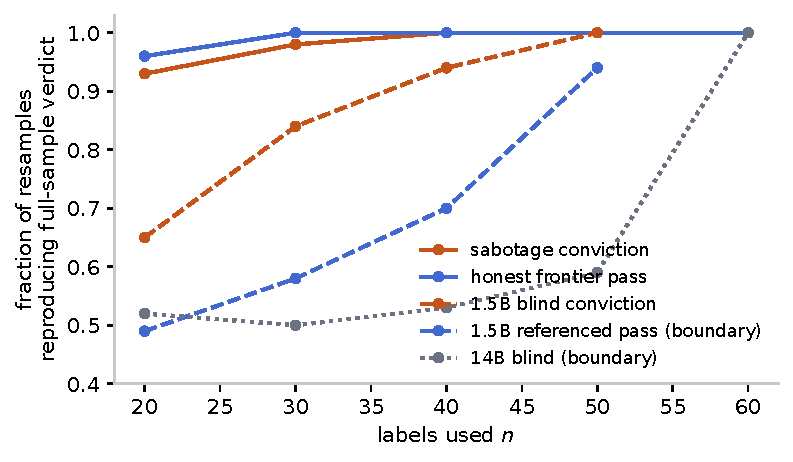
\includegraphics[width=0.62\textwidth]{figures/fig_stability.pdf}
\caption{\textbf{Takeaway: convictions are cheap and stable; verdicts near the pass boundary are the ones that need more labels --- and the one verdict that never stabilized below the full label set is the one that proved false.}
Verdict stability under label subsampling: fraction of 500 resamples per point reproducing the full-sample verdict under the fixed rules.}
\label{fig:stability}
\end{figure}

\paragraph{The convictions do not depend on the estimator, or on one rater grading both axes.}
Two post-hoc sensitivity analyses answer the two ways a partial correlation at $n \approx 60$ can mislead.
First the estimator: recomputing every configuration's loadings as rank (Spearman) partials, and again as standardized Huber-robust regression coefficients, leaves both nuisance verdicts intact (rank style partials $+0.56$ $[+0.34,+0.73]$ and $+0.53$ $[+0.31,+0.71]$; Huber style coefficients $+0.54$ and $+0.56$ against a maximum of $+0.17$ over every other configuration) and changes two verdicts, both at the pass boundary --- and one of the two it withdraws is the blind 14B, this record's false pass, which the rank estimator declines to certify.
Second the rater: because one annotator graded both axes, an error correlated across axes (``this looks wrong, so the writing feels muddled'') would manufacture exactly the structure the method reads.
Recomputing the partials on the 30-item overlap with the target axis from one rater and the nuisance axis from the other --- so no single person's halo can enter both --- the sabotage conviction is undiminished ($+0.61$ $[+0.28, +0.83]$ with author soundness and blind-rater style), the reward model reproduces in sign ($+0.41$ $[-0.01, +0.71]$), and the honest frontier stays clean ($-0.36$ $[-0.61, -0.20]$).
The cross-rater axis correlation is near zero ($-0.02$ and $+0.20$ across the two pairings, against $+0.28$ within the author's own labels), which is the direct measurement of the halo effect the design worried about: it is small.
A fully split-rater instrument, in which one hypothesis-blind pool grades soundness with the reference in view and a second grades style with no reference and no correctness question, is built and awaiting annotators; it is the version of this check we would run prospectively.

\paragraph{Why boundary passes must be abstained on.}
The label count and the rule interact, and a simulation calibrated to this instrument shows how.
Drawing target and nuisance labels with the measured cross-rater reliabilities ($0.83$ and $0.48$) and the anchor set's axis correlation, and drawing judges spanning the loading plane, the frozen point rule certifies a nuisance-loaded judge in $0.9\%$ of 60-label draws but a genuinely style-loaded-and-weak judge is caught in $93\%$; the cost sits on the other side, where a judge whose true target loading is $0.41$ --- the boundary case --- is certified in $46\%$ of draws at $n{=}60$ and still only $50\%$ at $n{=}240$, because the rule is asking a question the point estimate cannot answer.
The CI rule converts that coin flip into an abstention: it certifies the boundary judge in $2.9\%$ of draws and abstains in $43\%$, while losing almost nothing on clearly strong judges ($78\%$ certified at $n{=}60$, identical to the point rule).
The simulation says what the empirical record said: convictions are cheap, clear passes are cheap, and boundary passes are not purchasable at any label count this method can afford --- they must be abstained on.

\paragraph{How few labels suffice depends on the verdict.}
Convictions and strong passes stabilize with the fewest labels; boundary verdicts are the expensive ones.
Resampling the anchor set at fixed rules, the sabotage conviction reproduces in $0.93/0.98/1.00$ of draws at $n = 20/30/40$ labels and the honest frontier pass in $0.96/1.00/1.00$; the 1.5B-blind conviction reaches $0.94$ by $n{=}40$.
The boundary configurations differ from each other: the referenced-1.5B pass stabilizes by 50 labels ($0.94$ of resamples), while the blind-14B pass is still at $0.59$ at $n{=}50$ and reproduces only at the complete $n{=}60$ set --- and Section~\ref{sec:pressure} shows that this, the least stable verdict, is the false one (Figure~\ref{fig:stability}).
A few dozen labels certify clear cases; boundary verdicts honestly demand more.
The four-to-eight-hour figure is the labeling cost alone; end-to-end certification also requires assembling the trace pool, and the optional pressure backstop's generation and judge calls dwarf the labeling compute.

\paragraph{Toward zero labels, honestly scored.}
Two label-free extensions were registered, and they bracket what can be had for free.
A causal six-axis perturbation battery (length padding, reformatting, authority cues, bandwagon cues, confident-tone injection, and hedging, each preserving mathematical content and the final answer) confirms the honest frontier's registered insensitivity on all six axes and the blind 1.5B's registered positive presentation sensitivity (primary read $+0.65$; authority $+0.95$ $[+0.30, +1.75]$), and battery sensitivity rank-correlates with the audited style partials at Spearman $0.55$ against a registered bar of $0.5$ --- a pass of the registered test, not evidence of a strong effect, since the margin is thin at ten configurations.
The battery's sign prediction for the sabotaged judge, however, is falsified in direction: it is significantly sensitive on three axes but \emph{negatively} --- appended social cues and hedges lower its score (hedging $-0.53$ $[-0.72, -0.37]$) --- so it punishes any appended imperfection rather than rewarding authority; that is still a presentation sensitivity the honest judge lacks, but the registered sign was wrong, and we report it as promised.
A fully mechanical audit (machine correctness as target axis, log response length as the ignored axis, zero human labels) separates the two most corrupted evaluators by margin --- the sabotaged frontier and the reward model carry the two largest length-partial magnitudes ($-0.74$ and $-0.54$) with collapsed correctness partials --- but its pre-stated flagging rule also flags four other configurations, including two honest referenced passes, so the stated expectation that honest judges come out clean is partially violated.
The mechanical axes are a coarse screen that orders corruption severity, not a verdict instrument; the human-labeled audit remains the verdict tier.

\section{What the audit does not do}
\label{sec:limits}

\paragraph{Thirteen configurations are not thirteen independent tests.}
The audited configurations' verdicts are strongly collinear with one protocol bit, reference presence, and beyond it there are roughly four distinct verdict classes (blind-weak, referenced-pass, style-loaded, and sabotage-at-ladder-scale fail), so the validation is closer to four independent tests than thirteen; the ten-of-eleven count overstates the independent evidence, and the incremental-validity comparison of Section~\ref{sec:pressure} is the sharper statement of what the audit adds.
For the same reason we do not quote false-pass or false-convict rates: four effective classes cannot estimate them, and the registered replications (Putnam, the code audit) are what will accumulate the outcomes such rates require.
The two designed tests that break the collinearity --- the reward-model paraphrase replicate and the DPO experiment --- have both now run, and both confirmed their core registered claims.
A third was built for exactly this purpose and only partly succeeded: the prospective panel of Section~\ref{sec:panel} caught a referenced judge the protocol bit certifies, but its corrupt cells did not corrupt, so the audit's advantage over the bit there again rests on few cells.

\paragraph{One audited domain, anchored on math.}
The human-labeled audit was run once, on \textsc{MATH-500} solutions; code is a post-hoc extrapolation under a mechanical target axis, and the capability-gate explanation of its one miss is itself post hoc until the registered code audit runs.
The audit labels come from seventeen models' solutions while the primary pressure pools come from one generator, and all open-weights judges share that generator's family; the registered cross-family run closes the self-preference worry --- on a Llama-3.1-8B-generated pool (176 in-band items) the blind-versus-referenced separation replicates at every ladder size with disjoint intervals --- though the referenced tier is less clean cross-family (the 7B referenced inflation reaches $+0.50$, against at most $+0.18$ same-family), consistent with Qwen judges verifying Llama solutions less reliably.

\paragraph{The false pass is a boundary property the instrument cannot remove.}
Verdicts for judges near the pass line sit within interval overlap at these label counts, and the blind-14B false pass is that limitation realized rather than an anomaly: the subsampling analysis shows boundary verdicts are exactly the unstable ones.
The revised interval rule buys safety by abstaining there, at a measured cost of two correct certifications, and its record is retrospective until the Putnam replication scores it prospectively.

\paragraph{A correction to an earlier statement of the confound.}
Earlier drafts of this work described soundness and style as correlating at $+0.82$ in our labels.
That figure came from a twenty-item near-ceiling block graded early in the project, not from the sixty-item anchor set that carries every partial correlation reported here, where the two axes correlate at $+0.32$ $[+0.10, +0.55]$.
We state the corrected number and note what it does and does not change: the argument that marginal agreement cannot separate substance-reading from style-reading judges rests on the measured collision between the sabotaged frontier judge and the honest blind 14B (Table~\ref{tab:h2h}) and on the five-metric comparison of Table~\ref{tab:marginal}, neither of which depends on the size of the axis correlation; what a smaller correlation does change is the a priori case that the confound must be large, so we no longer make it.

\paragraph{The labels are noisy on precisely the convicting axis.}
Style reliability is $0.48$ cross-rater, the noisier of the two axes, which attenuates exactly the partials that carry convictions; the ceiling arithmetic is itself sensitive to the correlation measure (the soundness cross-rater Pearson of $0.83$ drops to a Spearman of $0.46$ at $n{=}30$), so the ceilings are indicative anchors, not walls, and the honest frontier's $+0.90$ soundness partial should be read as saturating what one rater's labels can measure.
The honest-frontier pass does not depend on the ceiling arithmetic.

\paragraph{The instrumented axes are a screen, not a perimeter.}
Style is the dominant documented nuisance axis and ours; length, format, and position were probed separately, and the six-axis battery probes further presentation cues synthetically.
An axis orthogonal to all instrumented ones can evade the audit, synthetic perturbations can be off-manifold, and outcome validation costs compute in every new domain; the pressure test is the axis-agnostic backstop, run per domain.
A pass also certifies outcomes, not process: with planted false steps that leave the final answer unchanged, frontier judges forgive $40$--$50\%$~\cite{companionB}.

\paragraph{Registration weight is uneven.}
Most registered-era predictions carry internal git timestamps on committed drafts and code, which establish ordering but cannot rule out selective disclosure; only the DPO rerun and the pending Putnam replication carry external OSF registrations with third-party timestamps.
The ledger in the technical report reports every registered prediction including the falsified ones, and the asymmetry is disclosed rather than repaired.

\section{Related work}
\label{sec:related}

The closest question to ours is whether any static measure predicts downstream optimization failure.
Benchmark accuracy does not~\cite{wen2024rethinking}; our contribution is a static, black-box, few-label measure whose frozen verdicts predicted the registered in-domain outcomes (Section~\ref{sec:pressure}), with a construct-validity design explaining why.
That design has a classical lineage: partial correlations against deliberately separated axes, with a positive control, is multitrait-multimethod construct validation~\cite{campbellfiske1959}, and the protocol-bit comparison follows standard incremental-validity practice; the contribution is bringing outcome-validated construct validity to judge deployments, not inventing the statistics.
Active auditing trains attackers against a frozen reward model~\cite{beigi2026ara}; the certificate needs no attacker, and the incremental-validity comparison shows what a no-attacker design detects beyond a protocol artifact: corrupted instructions and an off-the-shelf reward model.
Judge reliability audits measure consistency and bias robustness~\cite{judgechanges2026,zheng2023judging}; validity against decorrelated human axes, with a positive control, is the missing piece we add.
Style-over-substance biases are documented in general pools~\cite{wu2023style,dubois2024length,singhal2023long}, and style-substance conflation in trained reward models is established at the class level: RM-Bench finds the class fragile on curated style-controlled pairs~\cite{rmbench2024}, and reward-model benchmarks have been re-examined through the lens of overoptimization~\cite{kim2025lens}.
Those benchmarks characterize the evaluator class on fixed public data; the certificate is a per-deployment diagnostic with sign-anchored ex-ante conviction rules and validation against pressure outcomes on the same deployment distribution.
RM-Bench tells you the class is fragile; the audit tells you whether \emph{your} judge, on \emph{your} task and prompt, reads substance before you deploy it.
References are known to improve judge accuracy~\cite{refguided2024,smalljudges2025}; we show they flip audit validity, that the effect is capability-gated, and that on multi-valid tasks any reference harms statically~\cite{generous2026,dobefore2025} and amplifies gaming dynamically~\cite{companionD}.
Reward hacking is characterized post hoc~\cite{gao2022scaling,skalse2022defining,coste2023ensembles,eisenstein2023helping,selfplay2026}; the certificate is ex ante.
Companion work supplies the mechanism the audit instruments --- comparison-shaped signals grade the reference while verification-shaped signals grade the solution~\cite{companionB} --- and apparent evaluator failures in our own data dissolved, on adjudication, into evaluation-pipeline verdict errors, so the oracle should be audited before the evaluator~\cite{companionC}.

\section{Conclusion}

Raw agreement with human labels is not a certificate.
It measures performance on the observed unoptimized distribution and does not identify which correlated attributes of a response drive the score, and optimization risk depends on two of them: how much of the target a judge reads, and how much of a nuisance.
Weak judges fail on the first, capable-but-corrupt judges on the second, and raw agreement can see only the first.
An audit that reads both from the same labels predicts what the agreement rate cannot: a sabotaged frontier judge and an honest mid-size judge that raw agreement rates as interchangeable ($+0.35$ against $+0.37$) sit on opposite sides of a sign-anchored conviction rule; the frozen verdicts called the best-of-64 outcome for ten of eleven registered configurations, with the one false pass sitting $0.01$ above its cut and the revised interval rule abstaining there; on a prospective panel of nineteen judges it had never seen, the audit made no false certification, though that panel contained no successful corruption; and under externally registered DPO training the certified judge's arm gained real accuracy while the convicted judge's arm degraded it, the registered wedge prediction failing in the informative direction --- corruption expressed as damage, not gaming, at this scale.

The practical protocol is short.
Run the free screens first, since a judge that cannot agree with itself under order swap cannot be audited at all.
Then spend a few dozen blind labels on two separated axes, read the two partials, and apply the frozen rule: convictions are cheap, stable, and sign-anchored; passes near the boundary deserve more labels or an abstention, because the one verdict in this record that never stabilized below the full label set is the one that proved false.
Do not substitute raw agreement, which ranks but cannot diagnose; do not transfer a certificate across domains, since certification is a property of a judge, task, and prompt triple; and give a judge a reference only when the answer is unique and the judge can use it, because on multi-valid tasks the lever inverts~\cite{companionD}.
The audit costs four to eight annotator-hours against the price of discovering, after deployment, that the scoreboard was the only thing improving.

\enlargethispage{4\baselineskip}
{\small
\bibliographystyle{plain}
\bibliography{references}
}

\end{document}
